\section{Methodology}
\subsection{Data Preprocessing:}
\begin{itemize}
	\item Silence and Noise Removal\\
	Doing a spot check on both training and testing set, we discovered that there exists silence or noise at the beginning of most audio files. We removed those silence or noise parts by calculating the average loudness of each audio file, and recursively comparing the value of 30\% of average loudness to first $\frac{3}{4}$ of the audio file.\\
	\item Equalizing Loudness:\\
	We also figured out that ,between training set and testing sets, there is a loudness difference not representative of class label. So, we linearly equalized average loudness of each file by the average loudness of all audio files. \\
\end{itemize}
\subsection{Feature Extraction:}
\begin{itemize}
	\item Zero Crossing Rate(ZCR):\\
	The rate of sign-changes of the signal during the duration of a particular frame.\cite{b1}\\
	\item Energy:\\
	The sum of squares of the signal values, normalized by the respective frame length.\cite{b2}\\
	\item Entropy of Energy(EE):\\
	The entropy of sub-frames' normalized energies. It can be interpreted as a measure of abrupt changes.\cite{b2}\\
	\item Spectral Centroid(SC):\\
	It indicates where the "center of mass" of the spectrum is located. Perceptually, it has a robust connection with the impression of "brightness" of a sound.\cite{b3}\\
	\item Spectral Entropy(SE):\cite{b1}\\
	Entropy of the normalized spectral energies for a set of sub-frames.\cite{b3}\\
	\item Spectral Spread(SS):\\
	The second central moment of the spectrum.\cite{b3}\\
	\item Spectral Entropy:\\
	Entropy of the normalized spectral energies for a set of sub-frames.\cite{b3}\\
	\item Spectral Flux:\\
	The squared difference between the normalized magnitudes of the spectra of the two successive frames.\cite{b3}\\
	\item Spectral Rolloff:\\
	The frequency below which 90\% of the magnitude distribution of the spectrum is concentrated.\cite{b3}\\
	\item Mel Frequency Cepstral Coefficients(MFCCs):\\
	Mel Frequency Cepstral Coefficients form a cepstral representation where the frequency bands are not linear but distributed according to the mel-scale.\cite{b4}\\
	\item Chroma Vector:\\
	A 12-element representation of the spectral energy where the bins represent the 12 equal-tempered pitch classes of western-type music (semitone spacing).\cite{b5}\\
	\item Chroma Deviation:\\
	The standard deviation of the 12 chroma coefficients.\cite{b5}\\
	\item Local Amplitude Minimum:\\
	The number of local minimum amplitude peaks.\\
\end{itemize}
First 13 features are widely used in the field of machine learning for audio classification. We utilize an existing library\cite{b6} that implements first those features. The last feature Local Amplitude Minimum is introduced by us to help classifiers distinguishing normal audio and abnormal audio, which turns out to be extremely efficient. \\

\subsection{Model Selection:}
	Our whole model-building infrastructure is based on scikit-learn\cite{b2}\cite{b3}. \\
	We tried K-Nearest Neighbor, Support Vector Machine, Boosting, Random Forest, Extratrees, Multiple Instance Learning, Label Propagation. After few experiments, it seemed like tree algorithms performed poorly on this task and we finalized our focus on SVM, Label Propagation, SVC and MILR with pipeline. This classifier undercalled Normal and Neoplasm patients, which we think is resulted from different class distributions between training and testing set. So, we converted this relatively complex learning task into three less complicated tasks: Normal vs. Pathological, Vocal vs. Rest of Diseases, and Phonotrauma vs. Neoplasm.[Fig. 1.] The reason why we design the pipeline this way is based on the difficulty of classification. (From easiest Normal vs. Pathological to hardest Phonotrauma vs. Neoplasm)
	\begin{figure}[htbp]
		\begin{center}
			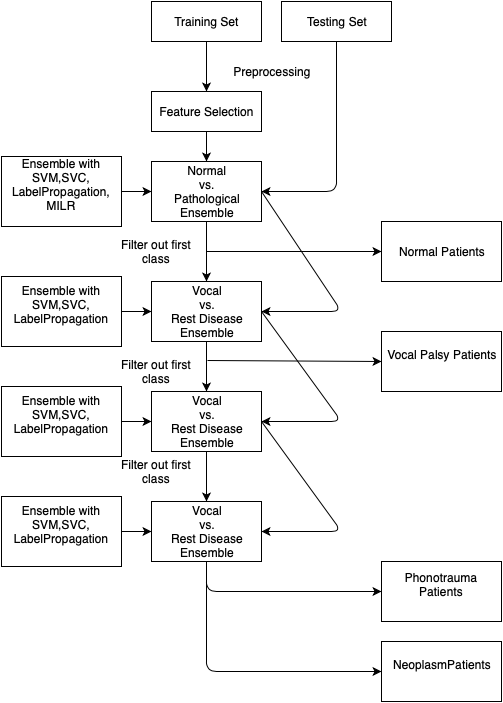
\includegraphics[scale=0.35]{Diagram_1.png}
		\end{center}
		\caption{Pipeline Ensemble}
	\end{figure}
	\subsection{Hyper Parameter Tuning:}
		Since the size of training set is getting smaller and smaller as we propagate through the pipeline, in order to get trustworthy accuracy to tune parameter for SVC, for all three ensembles, we use the same parameter tuned in the first ensemble. The process is pretty straightforward; we simply set up two loops, one of which for C and one of which for gamma. The tuned parameters are 10 for C, and 0.01 for gamma. Also due to the skewed distribution in training set, we modify the class weight with respect to the proportion of class. 

